\documentclass[border={0.1cm 0.1cm 0.1cm 0.1cm}]{standalone}  %E,S,W,N

\usepackage{amssymb}
\usepackage{amsmath}
\usepackage{tikz}
\usetikzlibrary{arrows.meta}

\begin{document}
	
	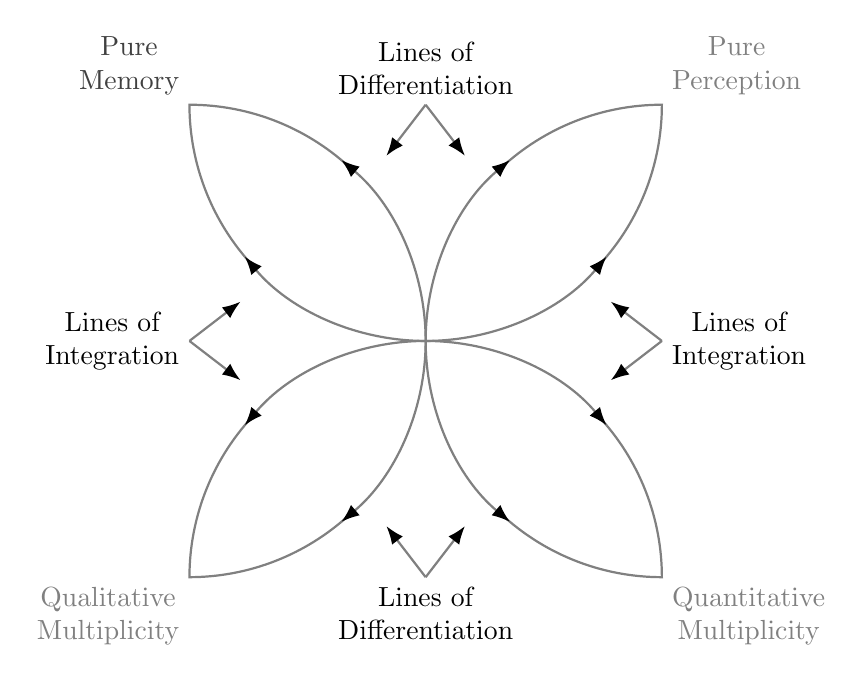
\begin{tikzpicture}[thick]	
	\draw[gray] ({-3+3*cos(46)},{3*sin(46)}) arc (46:90:3) arc (180:223:3);
	\draw[gray] ({3*cos(136)},{-3+3*sin(136)}) arc (136:180:3) arc (270:313:3);
	\draw[gray] ({3+3*cos(226)},{3*sin(226)}) arc (226:270:3) arc (0:43:3);
	\draw[gray] ({3*cos(316)},{3+3*sin(316)}) arc (316:360:3) arc (90:133:3);
	
	\draw[gray,<-<,arrows={-Latex[black,fill=black]}] (0,0) arc (270:220:3);
	\draw[gray,<-<,arrows={-Latex[black,fill=black]}] (0,0) arc (90:140:3);
	\draw[gray,<-<,arrows={-Latex[black,fill=black]}] (0,0) arc (270:320:3);
	\draw[gray,<-<,arrows={-Latex[black,fill=black]}] (0,0) arc (90:40:3);
	
	\draw[gray,->,arrows={-Latex[black,fill=black]}] (0,0) arc (0:50:3);
	\draw[gray,->,arrows={-Latex[black,fill=black]}] (0,0) arc (0:-50:3);
	\draw[gray,->,arrows={-Latex[black,fill=black]}] (0,0) arc (180:130:3);
	\draw[gray,->,arrows={-Latex[black,fill=black]}] (0,0) arc (180:230:3);
	
	%LABELS
	\node[darkgray,align=center,above left] at (-3,3) {Pure \\ Memory};
	\node[gray,align=center,above right] at (3,3) {Pure \\ Perception};
	\node[gray,align=center,below left] at (-3,-3) {Qualitative \\ Multiplicity};
	\node[gray,align=center,below right] at (3,-3) {Quantitative \\ Multiplicity};
	%
	\node[align=center,above] at (0,3) {Lines of \\ Differentiation};
	\node[align=center,left] at (-3,0) {Lines of \\ Integration};
	\node[align=center,right] at (3,0) {Lines of \\ Integration};
	\node[align=center,below] at (0,-3) {Lines of \\ Differentiation};
	
	%DIAGONAL ARROWS
	\draw[gray,->,arrows={-Latex[black,fill=black]}] (0,3)--++(-0.5,-0.65);
	\draw[gray,->,arrows={-Latex[black,fill=black]}] (0,3)--++( 0.5,-0.65);
	%
	\draw[gray,->,arrows={-Latex[black,fill=black]}] (0,-3)--++(-0.5,0.65);
	\draw[gray,->,arrows={-Latex[black,fill=black]}] (0,-3)--++( 0.5,0.65);
	
	\draw[gray,->,arrows={-Latex[black,fill=black]}] (-3,0)--++(0.65,0.5);
	\draw[gray,->,arrows={-Latex[black,fill=black]}] (-3,0)--++(0.65,-0.5);
	%
	\draw[gray,->,arrows={-Latex[black,fill=black]}] (3,0)--++(-0.65,0.5);
	\draw[gray,->,arrows={-Latex[black,fill=black]}] (3,0)--++(-0.65,-0.5);
	\end{tikzpicture}
	
\end{document}